\documentclass[twocolumn]{aastex62}

\newcommand{\vdag}{(v)^\dagger}
\newcommand\aastex{AAS\TeX}
\newcommand\latex{La\TeX}
\usepackage{amsmath}
\usepackage{physics}
\usepackage{hyperref}
\usepackage{natbib}
\usepackage[T1]{fontenc}
\usepackage[english]{babel}
\usepackage[utf8]{inputenc}
\usepackage{wasysym}

\begin{document}

\title{\Large AST5220-Milestone III: Evolution of Structure in the Universe}

\author{Nils-Ole Stutzer}

\begin{abstract}
    We have simulated the evolution of perturbations in the baryonic matter, dark matter and photons content of the Universe, as well as the metric potential perturbations over the Universe's history, by solving the coupled set of ordinary differential equations from the linearized Boltzmann and Einstein equations numerically. The monopole and dipole moments of the perturbations as well as the metric potentials were plotted against the log-scale factor $x = \ln a$, for different wavenumbers $k$. We could clearly see the acoustic oscillations in perturbations of scales that entered the causally connected Hubble sphere prior to matter-radiation equality at $a_\text{eq}$, both in the photon monopole and dipoles $\Theta_0$ and $\Theta_1$ as well as in the baryonic matter components $\delta_\text{b}$ and $v_\text{b}$, representing the interplay between gravity rarifying and radiation pressure expanding the perturbations. All superhorizon scale perturbations (matter or photons) entering late remained unchanged until their very late entry, while the smallest cold dark matter perturbations were suppressed by the Meszaros effect due to early horizon entry. The small scale metric potentials $\Phi$ and $\Psi$ decayed rapidly once entering the horizon, while superhorizon scales converged to $9/10$ of their initial value in the matter epoch being consistent with \cite{dodelson:2003}. In general all results seemed to be consistent with known physics and external results, and are hence concluded to be significant.


    \textit{The codes for this paper can be found at:} \newline \url{https://github.com/SagittariusA-Star/AST5220-Milestones}
\end{abstract}

\section{Introduction} \label{sec:Intro}
Nowadays cosmology is considered a high precision field of science, a status which cosmology gained through high precision measurements of the Cosmic Microwave Background (CMB) with several telescopes and probes, Planck \citep[]{planckcollaboration:2018} being the most significant to date. Planck's measurements of the CMB anisotropies have led to a revolution in cosmology, as the accurate measurements can be used to estimate cosmological parameters and subsequently tightly constrain cosmological models of the universe we live in.

In order to estimate cosmological parameters one needs to first model the CMB. This paper is a step towards the final goal of computing the angular CMB anisotropy power spectrum of temperature perturbations at the surface of last scattering (LSS). We will continue the work of \cite{stutzer:2020a} and \cite{stutzer:2020b} by further building on the model of the universe by implementing the perturbations that ultimately form the anisotropies of CMB. We will do this by solving the coupled set of differential equations (ODEs) of the multipole moments of the radiation, cold dark matter (CDM) and baryonic matter, neglecting neutrinos and the polarization of photons for simplicity. Also we only consider hydrogen to make up the baryons, an approximation which should hold fairly well, as hydrogen is the dominant species of baryons. These multipoles for the different perturbations can subsequently be used to compute the theoretical CMB power spectrum for a set of cosmological parameters (future work).

\section{Method} \label{sec:Method}
The equations and relations presented here are, unless otherwise stated, provided by \cite{callin:2006}, \cite{winther:2020b} and or \cite{dodelson:2003}. We thus refer to these authors for detailed derivations, as we will merely present the main path towards solving for the evolution of the perturbation.

\subsection{The System of Equations} \label{subsec:system}
After having modeled the large scale evolution of the universe and its recombination history, we can add the small inhomogeneities of matter-energy of photons, CDM and baryonic matter and compute their evolution over time as a function of scale. The evolution of the perturbations for different scales are found by solving the linearized Einstein and Boltzmann equations in Fourier space with the initial conditions set up by inflation, which are derived in detail in \cite{dodelson:2003} and presented by \cite{winther:2020b}. In principle this is merely a system of coupled ODEs which have to be solved for. However, there are some difficulties. Since the universe was hot and dense at early times, an electron would only "see" a short distance, and hence could only be affected by nearby temperature fluctuations. This is seen from the large optical depth at early times as found by \cite{stutzer:2020b}. Since the system was effectively in thermodynamic equilibrium with only small fluctuations, only the first few multipoles are relevant for the evolution of the photon-baryon plasma at early times. The relevant multipoles are the monopole $\Theta_0$ representing the average temperature of the electron, the dipole $\Theta_1$ which can roughly be thought of as the radial velocity of the density perturbation and the quadrupole $\Theta_2$ which is the only relevant source for polarization (which we will otherwise neglect) this early on \citep[]{winther:2020b}. This early regime is called tight coupling, where matter and radiation forms a tightly coupled plasma.

Later on the universe became optically thinner and multipoles $\Theta_\ell$ of higher orders became relevant. In principle, since the ODEs for the multipoles of different order are all coupled, one needs to solve for a high number of these coupled equations. As this is highly inefficient, we make use of the line of sight integration developed by Zaldarriaga and Seljak later on when computing power spectra, for which only needs a few (eight) of the multipoles. We thus truncate the system of equation at eight.

Since we, as mentioned in Sec. \ref{sec:Intro}, only consider photons, CDM and baryonic matter perturbations we get the following differential equations for the photon multipole moments

\begin{align}
    \Theta^\prime_0 &= -\frac{ck}{\mathcal{H}} \Theta_1 - \Phi^\prime, \\
    \Theta^\prime_1 &=  \frac{ck}{3\mathcal{H}} \Theta_0 - \frac{2ck}{3\mathcal{H}}\Theta_2 +
    \frac{ck}{3\mathcal{H}}\Psi + \tau^\prime\left[\Theta_1 + \frac{1}{3}v_b\right], \\
    \Theta^\prime_\ell &= \frac{\ell ck}{(2\ell+1)\mathcal{H}}\Theta_{\ell-1} - \frac{(\ell+1)ck}{(2\ell+1)\mathcal{H}}
    \Theta_{\ell+1} \nonumber \\
    &+ \tau^\prime\left[\Theta_\ell - \frac{1}{10}\Pi
    \delta_{\ell,2}\right], \qquad  2 \le \ell \leq \ell_{\textrm{max}} \\
    \Theta_{\ell}^\prime &= \frac{ck}{\mathcal{H}}
    \Theta_{\ell-1}-c\frac{\ell+1}{\mathcal{H}\eta(x)}\Theta_\ell+\tau^\prime\Theta_\ell,
    \quad\quad \ell = \ell_{\textrm{max}},
\end{align}
The first two moments of which can be thought of as the density and the velocity perturbation respectively. We let $\ell_\mathrm{max} = 8$ for a total of eight multipole moments for photons. The scaled Hubble parameter $\mathcal{H}$ and the conformal time $\eta$ are computed in \cite{stutzer:2020a}, and the optical depth $\tau$ and its derivative $\tau^\prime$ are computed in \cite{stutzer:2020b}. The polarization tensor $\Pi = \Theta_2$ if polarization is neglected. The scale, of which every perturbation is a function of, is given by the wavenumber $k$ which is the inverted scale of the perturbation and the light speed is $c$ (all units are in the SI system). 

The perturbations to the CDM and baryonic matter-energy field are given by 
\begin{align}
    \delta_{\rm CDM}^\prime &= \frac{ck}{\mathcal{H}} v_{\rm CDM} - 3\Phi^\prime \\
    v_{\rm CDM}^\prime &= -v_{\rm CDM} -\frac{ck}{\mathcal{H}} \Psi \\
    \delta_b^\prime &= \frac{ck}{\mathcal{H}}v_b -3\Phi^\prime \label{eq:v_cdm}\\
    v_b^\prime &= -v_b - \frac{ck}{\mathcal{H}}\Psi + \tau^\prime R(3\Theta_1 + v_b), \label{eq:v_b}
\end{align}
where the density perturbations for CDM and baryons are given by $\delta_\mathrm{CDM}$ and $\delta_b$ respectively being the monopole moment of the matter components. The dipole moment of perturbations of the two matter components, i.e. the velocity perturbations are given by $v_\mathrm{CDM}$ and $v_b$. The factor $R = \frac{3\Omega_{r,0}}{4\Omega_{b,0}a}$, where $a$ is the scale factor.

And finally the perturbations to the time-time and space-space components of the metric (in the Newtonian gauge) are given as 
\begin{align}
    \Phi^\prime &= \Psi - \frac{c^2k^2}{3\mathcal{H}^2} \Phi
    + \frac{H_0^2}{2\mathcal{H}^2}
    \bigl[\Omega_{\rm CDM,0} a^{-1} \delta_{\rm CDM}\\
    & + \Omega_{b,0} a^{-1} \delta_b + 4\Omega_{r,0}
    a^{-2}\Theta_0 \bigr] \label{eq:Phi}\\
    \Psi &= -\Phi - \frac{12H_0^2}{c^2k^2a^2}\left[\Omega_{r,0}\Theta_2\right].\label{eq:Psi}
\end{align} 
Through Einstein's field equations one can see that the matter-energy content of the universe and the space-time curvature are determined by each other, and hence the perturbations of the matter-energy components (photons, CDM and baryons) will result in these metric perturbations. 
Note that in fact only one of the two metric perturbations is dynamical, meaning we don't have to solve for $\Psi$ as an ODE as it is determined by $\Phi$ and $\Theta_2$ directly.
Because these metric perturbations are perturbations to the curvature of space-time caused by the presence of a matter-energy perturbation, they will define the gravitational potential wells that matter and radiation can fall into or oscillate in under influence of pressure. 

As mentioned before there is however a slight complication in that the universe was hot and dense in the beginning, with a tight coupling between matter and radiation. In the tightly coupled regime $\tau'$ is large and $\Theta_1$ and $v_b$ are close to zero. Thus the factor $\tau' (3\Theta_1 + v_b)$ becomes numerically very unstable early on. Therefore one needs to do an approximation, derived in detail by \cite{callin:2006} and \cite{winther:2020b}, where we define the term 
\begin{align}
q &= \bigr(-[(1-R)\tau^\prime + (1+R)\tau^{\prime\prime}](3\Theta_1+v_b) \\&-
            \frac{ck}{\mathcal{H}}\Psi + (1-\frac{\mathcal{H}^\prime}{\mathcal{H}})\frac{ck}{\mathcal{H}}(-\Theta_0 +
            2\Theta_2) \\ &- \frac{ck}{\mathcal{H}}\Theta_0^\prime\bigr)/\bigl((1+R)\tau^\prime + \frac{\mathcal{H}^\prime}{\mathcal{H}} -
            1\bigr)
\end{align}
which is used to get more numerically stable expressions given as 
\begin{align}
    v_b^\prime &= \frac{1}{1+R} \left[-v_b - \frac{ck}{\mathcal{H}}\Psi + R(q +
    \frac{ck}{\mathcal{H}}(-\Theta_0 + 2\Theta_2) - \frac{ck}{\mathcal{H}}\Psi)\right]\\
    \Theta^\prime_1 &= \frac{1}{3} (q - v_b^\prime).
\end{align}
The ODEs for the monopole $\Theta_0$, as well as for $\delta_\mathrm{CDM}$, $v_\mathrm{CDM}$ and $\delta_b$ in the tightly coupled regime are simply the same as outside tight coupling as defined earlier.
Apart from the above rewriting for numerical stability sake, the only difference from the full equations, valid outside of tight coupling, is that one only needs to solve ODEs for the first two multipole moments $\Theta_0$ and $\Theta_1$ (and the CDM and baryonic quantities) since all other $\Theta_\ell$ are directly determined by the two former. Specifically without considering polarization the multipoles are given by
\begin{align}
    \Theta_2 &= 
    -\frac{20ck}{45\mathcal{H}\tau^\prime} \Theta_1, \quad\quad \textrm{(without polarization)}\\ 
    \Theta_\ell &= -\frac{\ell}{2\ell+1} \frac{ck}{\mathcal{H}\tau'} \Theta_{\ell-1}, \quad\quad \ell > 2.
\end{align}
Now that all equations for the tightly coupled regime are set up, we only need initial conditions before solving the system of ODEs in this regime. The initial conditions are set up by inflation an are as shown in \cite{winther:2020b} and \cite{callin:2006} given by 
\begin{align}
    \Psi &= -\frac{2}{3}\\
    \Phi &= -\Psi \\
    \delta_{\rm CDM} &= \delta_b = -\frac{3}{2} \Psi \\
    v_{\rm CDM} &= v_b = -\frac{ck}{2\mathcal{H}} \Psi\\
    \Theta_0 &= -\frac{1}{2} \Psi \\
    \Theta_1 &= +\frac{ck}{6\mathcal{H}}\Psi \\
    \Theta_2 &= 
    -\frac{20ck}{45\mathcal{H}\tau^\prime} \Theta_1, \quad\quad \textrm{(without polarization)}\\
    \Theta_\ell &= -\frac{\ell}{2\ell+1} \frac{ck}{\mathcal{H}\tau^\prime} \Theta_{\ell-1}.
\end{align}
In fact due to the system of equations being linear one can later pick a different initial condition for $\Psi$, and simply propagate the change through the other equations if other normalizations are desired. 

To integrate the perturbations over the entire history of the universe through today, we must finally determine how to transition from the system of the tightly coupled regime to the full set of equations. The time $x_\text{end of tc}$ of transition is essentially when $|\dv{\tau}{x}| < 10 \cdot \mathrm{min}(1, \frac{ck}{\mathcal{H}})$, but no later than the very beginning of recombination at $z\approx 1700$ which corresponds to $X_e\approx 0.999$ from \cite{winther:2020b}. This transitioning time must be found for each scale $k$ individually. 

After determining the time of transition, initial conditions for the full system are needed in order to solve the ODEs. These initial conditions are simply the values of the quantities at the time right before transition, i.e. the last values in the regime of tight coupling. Thus the tightly coupled regime must be treated first in order to initialize the full system. 

Some of the things we expect to see in the final solutions are the monopole moment of the photon-baryon plasma to oscillate in the gravitational potentials before decoupling happens. This is the interplay between the radiation pressure expanding a perturbation and gravity pulling collapsing it, together forming an oscillatory interplay. After matter and radiation decouple, the photons can free-stream, and the perturbations are frozen in on the LSS as the CMB anisotropies. We also expect different scales to perform differently. Small scales would enter the Hubble horizon earlier and only start growing or oscillating under gravity and pressure once they enter, while large super horizon scales entering late or not at all would stay unchanged. Small scales well below the sound horizon (the scale a sound wave could have traveled at a given time) at decoupling $r_* = \int^{\eta_*}_0 c_s d\eta$, for sound speed $c_s$, have the chance to performed more oscillations than scales just barely within the sound horizon. Scales above the sound horizon have not even had the chance to perform a single oscillation within the time of decoupling.

The matter density perturbations $\delta$ should reproduce the known plots of the Meszaros suppression, where the perturbations grow as the scale factor $a$ squared prior to matter-radiation equality $a_\text{eq}$, while being suppressed to grow as $\ln a$ after entering the horizon prior to $a_\text{eq}$ as discussed by \cite{dodelson:2003}. After $a_\text{eq}$ we then expect to see perturbations to grow proportional to the scale factor \citep[]{dodelson:2003}. Further we expect to see the smaller perturbations to enter the horizon earlier, hence the large scales (i.e. larger k) should be suppressed more. 

The scale dependence of the metric perturbations should also be seen. Prior to horizon entry the potentials $\Phi$ and $\Psi$ should start out equally in size but with opposite signs. They should behave as constants when outside the causally connected horizon defined by the Hubble sphere. When entering the horizon, the whole perturbation is causally connected, and the expanding universe will lead to the potential wells given by $\Phi$ and $\Psi$ to "flatten", reducing the well's "depth". This is seen by $\Phi$ and $\Psi$ decaying, symmetrically, towards a constant level after entering the horizon. The super horizon potentials will also slightly decrease, nevertheless remain quite flat, approaching 9/10 of their initial value \citep[]{dodelson:2003}.  

These are just some of the expectations to look out for, but there could of course be more interesting things to discover in the final results.

\subsection{The Implementation} \label{subsec:implementation}
Now that the system of ODEs is set up, we are ready to solve it using C++. The main idea of solving is that we want to loop through different scales $k$ and for each iteration solve the system of ODEs through time $x$. We use logarithmically spaced values for the wavenumbers $k$ to loop through. Inside each iteration of the $k$-loop we fist find the time $x_\text{end of tc}$ when tight coupling ends. This time is used to divide the timeline $x$ into two, one for each regime. In the first regime the initial conditions are set at described in \ref{subsec:system} as set up by inflation. The ODEs for tight coupling are solved and the quantities depending on those (i.e. the higher order multipoles) are computed, after which the results are saved in $n_x\times n_k$ matrices for later use.

Similarly the second half of the time axis, after transitioning outside the tight coupling, the full system of ODEs are solved with the initial conditions being the last values of tight coupling. The results are subsequently saved in the $n_x\times n_k$ grid matrices. The system of ODEs in each regime is solved using the \texttt{ODEsolver}-routine provided by \cite{winther:2020b}. The reason for dividing the ODE system in two, instead of solving the whole system in on go, is that the number of dynamical equations (i.e. ODEs) is different in the two regimes. Hence two separate ODE objects are needed for solving. 

Finally, before plotting the final outputs, spline interpolations of the saved $n_x\times n_k$ grid values of the solved quantities are made, so as to make a more continuos representation of each quantity. For that the \texttt{Spline2D}-routine by \cite{winther:2020b} is used. The very final output for plots are saved in data files, and plots are made from those in Python.

\begin{figure*}
    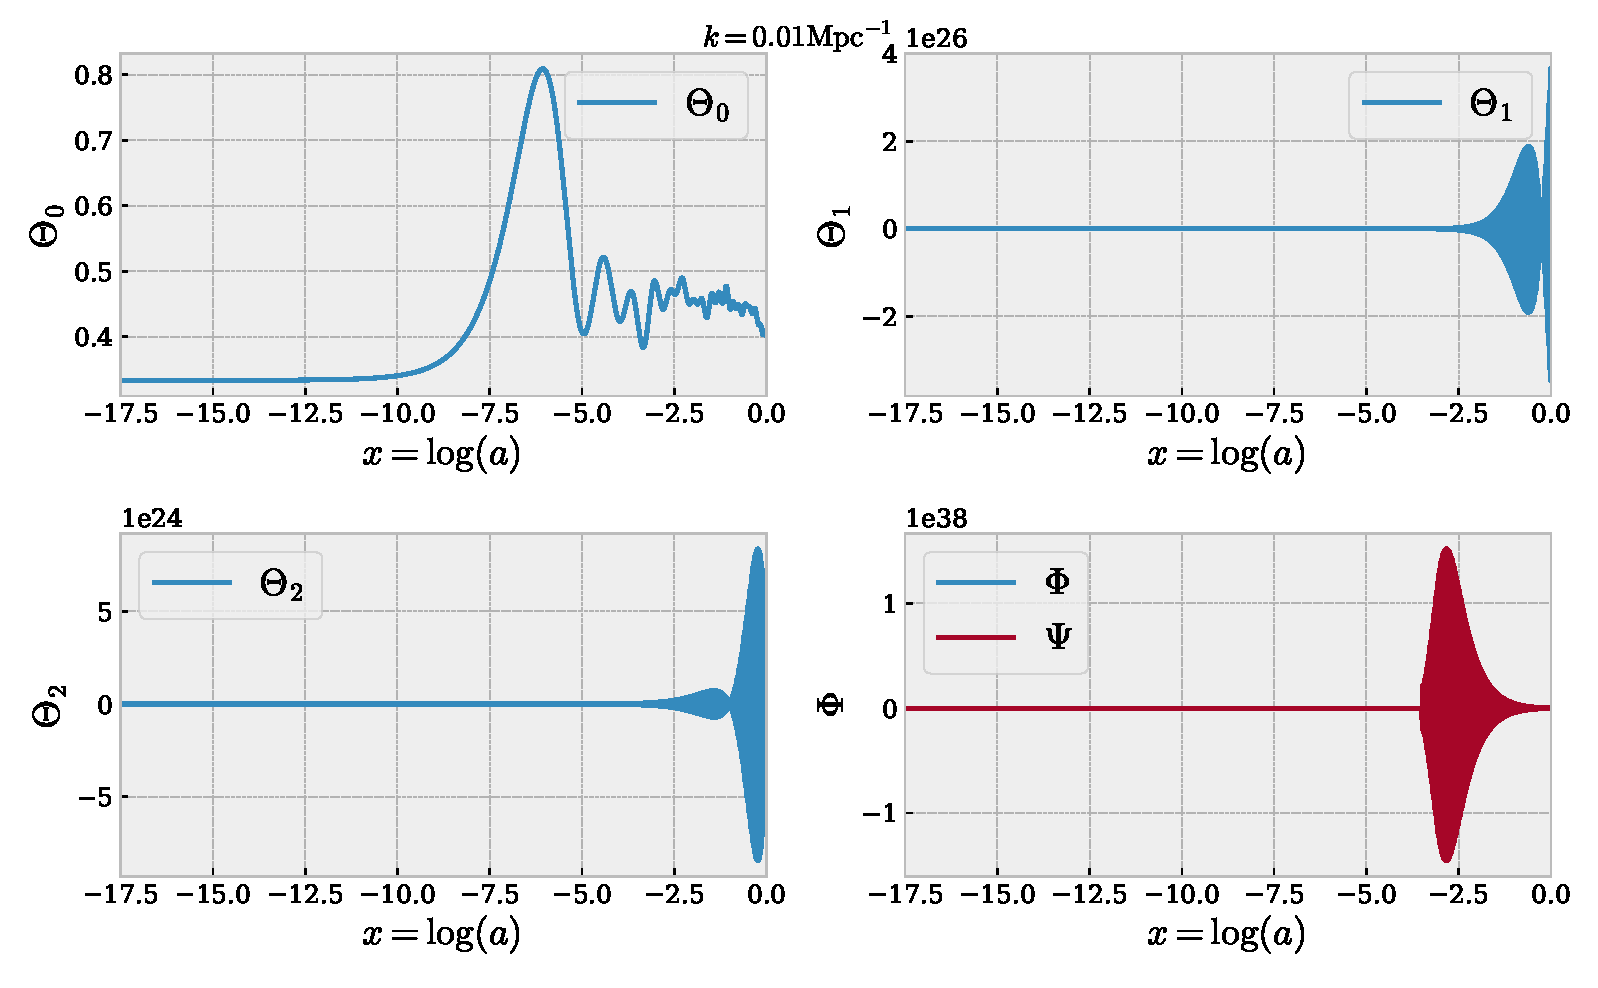
\includegraphics[scale = 0.65]{Figures/fig1.pdf}
    \caption{The figure shows (\textbf{Upper left}) the monopole moment $\Theta_0 = \frac{1}{4}\delta_\gamma$ and (\textbf{upper right}) the dipole moment $\Theta_1 = -\frac{1}{3}v_\gamma$, roughly corresponding to the density and velocity perturbation of radiation energy-density perturbation respectively. Also shown (\textbf{lower right}) are the metric perturbations $\Phi$ and $\Psi$ in the Newtonian gauge. All quantities plotted are functions of the log-scale factor $x = \ln a$ and scale $k$, and are shown for several different wavenumbers. The background color marks the epoch of dominance; yellow, blue and purple represent radiation, matter and dark energy dominated epochs respectively. The red background color corresponds to the epoch of recombination, given by the width of the peak of the visibility function from \cite{stutzer:2020b}, and the vertical red dash-dotted line represents the time of matter-radiation equality. Dotted vertical lines mark the time of horizon entry for a given scale, except for the largest scale, which enters after today.} 
    \label{fig:fig1}
\end{figure*}

\begin{figure*}
    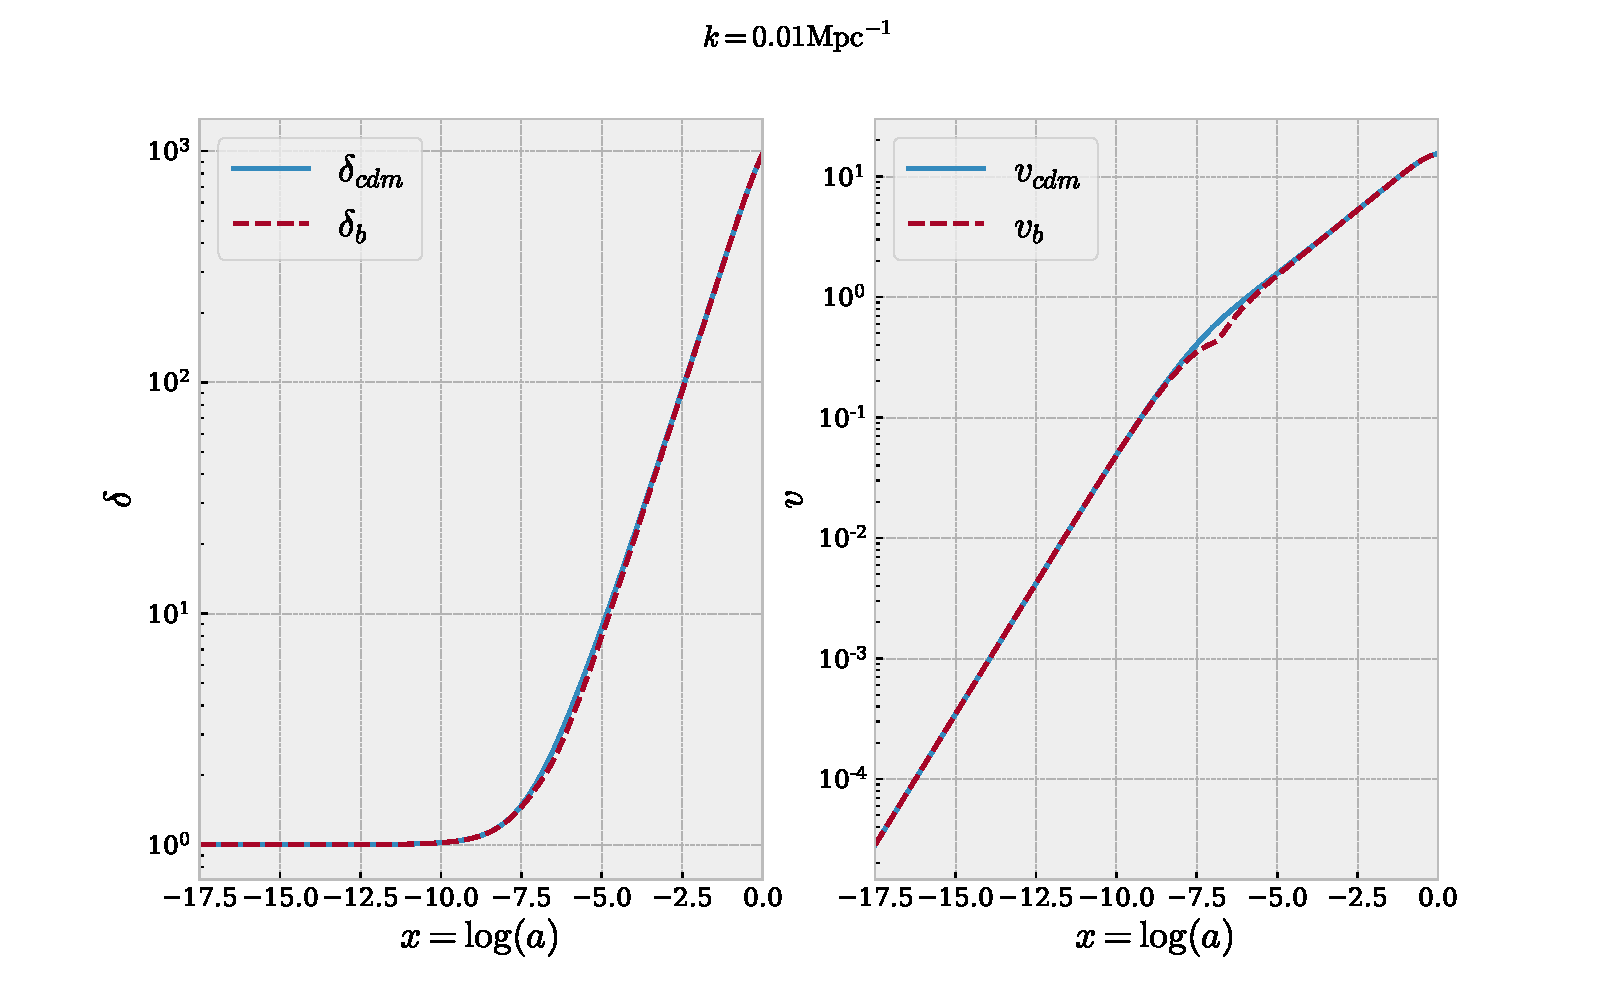
\includegraphics[scale = 0.65]{Figures/fig2.pdf}
    \caption{The \textbf{upper left} panel shows the density perturbations of the dark and baryonic matter perturbations (solid and dashed lines respectively). The \textbf{upper right} panel shows the velocity perturbations for dark and baryonic matter (same meaning of line style as in the left panel). The \textbf{lower} panel shows the co-moving density contrast of dark matter only. The scales $k$ of the perturbations described by the legend correspond to all of the three plots. The quantities shown are functions of the log-scale $x = \ln a$.  The background color marks the epoch of dominance; yellow, blue and purple represent radiation, matter and dark energy dominated epochs respectively. The red background color corresponds to the epoch of recombination, given by the width of the peak of the visibility function from \cite{stutzer:2020b}. Dotted vertical lines mark the time of horizon entry for a given scale, except for the largest scale, which enters after today.}
    \label{fig:fig2}
\end{figure*}

\section{Results}\label{sec:Results}

After having run the simulation computing the perturbations evolution throughout time, we end up with the plots seen in Figure \ref{fig:fig1} and Figure \ref{fig:fig2}.

In Figure \ref{fig:fig1} one can see the first two multipole moments $\Theta_0$ and $\Theta_1$ of the photon perturbations in the upper panels, as well as the two metric perturbations in the lower panel, all as functions of the log-scale factor $x$. In the lower panel the time-time and space-space components of the metric perturbations are marked with solid and dashed lines respectively. In each plot one can see the evolution of the respective quantity for six different scales, given by the wavenumber $k$ in the legend, spanning from sub to superhorizon scales. The color code in the background represent the respective epochs of dominance (i.e. radiation, matter and dark energy eras, see caption for details) as well as the epoch of recombination. The width of the latter one corresponds roughly to the width of the peak of the visibility function computed in \cite{stutzer:2020b}. 

In Figure \ref{fig:fig2} we see the density perturbations of the CDM and baryon components of the matter in the upper left panel and the corresponding velocity perturbations in the upper right panel. Again the CDM and baryon graphs are marked with solid an dashed lines respectively. The lower panel shows the co-moving (gauge invariant) dark matter density perturbation. The same six wavenumbers are used to produce these results as for the ones presented in Figure \ref{fig:fig1} and the legend of the lower panel shows which graph each wavenumber corresponds to. The same background color code used in Figure \ref{fig:fig1} is used in Figure \ref{fig:fig2}. vertical dotted lines show the horizon entry for each respective scale.

Note that all quantities shown are in Fourier space, not position space. Hence the velocity perturbations of the matter components can actually be greater than unity, as they are not directly to interpret as the real space velocities.

\section{Discussion}\label{sec:Discussion}
When looking at the plots of the upper two panels in Figure \ref{fig:fig1} we see the monopole and dipole moments of the radiation perturbations. When looking at, for instance, the monopole moment of the upper right panel, we see also the different behaviour of the perturbations on different scales. The largest scales, larger than the horizon at matter-radiation equality $k\ll k_\text{eq} \approx 0.00523 /\mathrm{Mpc}$, stretching outside the Hubble sphere $r = c/H$ remain basically unaffected for the entire history of the universe. That is because these perturbations are larger than the causally connected region on which gravity and pressure could act, resulting in no growth or decrease in density or velocity as long as being prior to horizon entry.

On the very small scales, smaller than the horizon at matter-radiation equality $k \gg k_\text{eq}$, e.g. $k = 0.3 /\mathrm{Mpc}$ and $0.0527 /\mathrm{Mpc}$ (see yellow and black curves), the behaviour of perturbations look quite different. Prior to horizon entry (the times of entry is marked by the dotted vertical line for a given scale) the large and small scale modes behave the same, just being constant. However, once entering the horizon prior to equality, we see $\Theta_0$ behaves highly oscillatory. These oscillations are the so called acoustic oscillations of the matter-radiation plasma (as matter and radiation are highly coupled prior to recombination). The oscillations basically show the interplay between gravity, which contracts the perturbations rarifying them, and the pressure forces by the enormous radiation pressure expanding the perturbations. Once having entered the horizon a perturbation grows rapidly, i.e. the density given by the monopole $\Theta_0$ grows when the perturbation accretes more plasma falling into the gravitational well set up by the perturbation. When the plasma falls in to the potential well, the radiation pressure increases, gradually slowing down the growth in $\Theta_0$, eventually able to counteract the pull of gravity completely. This expansion leads to the perturbation shrinking in density again. Once the blob has expanded it cools down, and the whole cycle starts over again resulting in the oscillatory behaviour seen. This is basically how sound waves in the primordial photon-baryon plasma look like in Fourier space.

The oscillations or relativistic sound waves on these small scales keep on going until the epoch of recombination. At that time the radiation and baryon decouple and the photons can free stream out of any potential wells. Thus the oscillations effectively stop as the photons travel freely, not being bound in the dense plasma anymore. We see exactly this happening in the plots, where the oscillating perturbations decay rapidly as they cross the epoch of decoupling. Further more, it is these free streaming photons that give rise to the CMB we see today. Hence the anisotropies seen in the CMB are the frozen-in picture of the photons at their last oscillation before decoupling. In fact the perturbations that perform one half expansion, i.e. collapse to the point right before subsequent expansion, within the time of recombination $x_*$ form the first peak of the acoustic oscillation pattern in the later-to-be computed CMB angular power spectrum and their scale defines the sound horizon at decoupling. This corresponds about to the $k = 9.24\cdot 10^{-3}/\mathrm{Mpc}$ scale monopole in our case (in fact slightly lower scale, but as seen in the plot this is the closest one we have computed). Similarly the other peaks of the CMB power spectrum are perturbations having performed multiples or halves of oscillations at the time of decoupling, and the troughs of the power spectrum are formed by the perturbations crossing the zero line in their oscillation at $x_*$.

Notice also that smaller among the small scale perturbations perform more oscillations than the somewhat large ones (the yellow and black curves in Figure \ref{fig:fig1}). This is due to two effects, the first of which is the basic fact that smaller scales enter the horizon earlier and can hence start growing under gravity earlier. The second reason is that pressure (waves) that travel with the sound speed of the medium $c_s$ ($\sim c$ early on) will take longer to establish pressure against gravity in a larger scale perturbation. This effect is somewhat analogous to classical causality (we could call it "acoustic causality"), where for instance gravity can only travel at the speed of light. Also, this might be the reason for why the oscillation peaks of $\Theta_0$ for $k = 0.3/\mathrm{{Mpc}}$ are slightly narrower than the once of $k = 0.0527/\mathrm{Mpc}$. 

The behaviour of the dipole $\Theta_1$ seems to correspond well to the behaviour of the monopole $\Theta_0$. As the dipole can be interpreted as the radial velocities of a perturbation blob, we expect to see a relative phase shift compared to the monopole, when looking at the oscillations performed for small scales entering prior to equality. This is because the oscillating quantity ($\Theta_0$ in this case) is always at its maximum speed when passing zero (or rather equilibrium) in an oscillation, while if at an extremal point in the oscillation the velocity is always zero (point of turn-around). This is exactly what we see, for instance the $k = 0.3/\mathrm{Mpc}$ perturbation having a peak in $\Theta_0$ where $\Theta_1$ has a zero at $x\sim-10$.

Next we consider the metric potential perturbations seen in the bottom panel in Figure \ref{fig:fig1} for different scales. Immediately we see that, as expected, the time-time and space-space components of the metric perturbations behave exactly symmetrically w.r.t. each other around the zero line. This is easily seen from (\ref{eq:Psi}) in the absence of anisotropic stress, i.e. for small $\Theta_2$, we simply get $\Psi = -\Phi$. The next tendency we notice is that the larger scale a perturbation has the "flatter" the corresponding potentials become throughout time. This is again an effect of the larger wavenumbers stretching outside the Hubble sphere. According to Dodelson \cite[p. 191]{dodelson:2003} we should expect the late time potential for large scales to approach $9/10$ of the initial value. As one can see in Figure \ref{fig:fig1}, we see this convergence when decreasing $k$ (note that the two largest scales are overlapping). Thus a potential well of a certain "depth" will remain as it is as long as it is outside the horizon. Superhorizon scales that don't enter the horizon until relatively recently or even after the current epoch, will thus remain quite flat, only decrease a little due to transitioning into the matter epoch. 

For the metric perturbations on the smallest scales we see that they start out flat too at early times. However, at a certain time, which corresponds to the time where the scale of the perturbation $k$ matches the horizon, the perturbation enters the horizon and starts decaying. That is because a potential well on subhorizon scales are being affected by the large scale evolution of the universe. When the potential well is stretched out it decreases in "depth" until it effectively vanishes or approaches a new constant level. Note also that we again see the very smallest perturbations starting their decay earlier than the larger ones, due to smaller perturbations entering the horizon earlier. 

At late times we see the potentials again decaying, which is due to the dark energy causing an exponential growth of the universe, rapidly decreasing the potentials. This is also what makes the very largest scale perturbations in $\Theta_0$ grow a little at late times. Free streaming photons that fall into the potential well, will get boosted in energy. But as they climb out again the potential well has decreased due to expansion of space, thus robbing the photon of less energy than it gained from falling into the well in the fist place. Thus the photon is net boosted in energy. This is the so called (Late) Integrated Sachs-Wolf effect (ISW).

The last little detail in the plots of the potentials we point out is the oscillatory behaviour of the potential for $k = 0.3/\mathrm{Mpc}$ after horizon entry and before recombination. At fist look, one may think this is somehow related to the acoustic oscillations see in $\Theta_0$ and $\Theta_1$, and in fact this initial suspicion is correct. As shown by \cite{dodelson:2003} and can be seen by eq. \ref{eq:Phi}, for a neglegible $\Phi'$ after horizon entry $ck \ll \mathcal{H}$, we expect $\Phi \propto \Theta_0 / \eta^2$, since $c/\eta = \mathcal{H}$ in the radiation era. Therefore we see the damped oscillations of $\Theta_0$ in the potentials, which intuitively can be understood by an oscillating source term causing an oscillating potential.

Next we consider the results of Figure \ref{fig:fig2} where we start with the upper left panel. As mentioned before this plot shows the density contrast for CDM and baryons for different scales as they evolve in time. Before going into detail, it is useful to note that these quantities are not gauge invariant, and hence only look this particular way in the Newtonian gauge which we used. However, the expected behaviour of the density contrast is known and we compare it to the once provided by \cite{dodelson:2003}. 

The first thing one perhaps notices when looking at the density contrasts is that again nothing special happens before the perturbation has entered horizon. The reason again being that the whole perturbation is not yet causality connected, inhibiting gravity to collapse the blob, hence letting the density stay constant. This is especially noticeable in the $k = 5\cdot 10^{-5} / \mathrm{Mpc}$, which is a superhorizon scale the whole time and thus remains untouched by gravity. This is a common feature among large and small perturbation for both CDM and baryons as seen in the plots. 

However, the point of horizon entry is where the scale of the perturbations matter. We see that the largest perturbations that enter late after equality, go from a constant density contrast to a linear growth where $\delta\propto a$ (for CDM and baryons) which is well in accordance with \cite{dodelson:2003}. For these large scale perturbations the CDM and baryon matter perturbations behave basically exactly the same. If however, the perturbations are smaller than the horizon at equality $\eta_\text{eq}$ and enter prior to the matter epoch something different happens. If we consider the $k = 0.3 /\mathrm{Mpc}$ perturbation we see that after entering in the radiation era at $x\sim-11.5$, the CDM density grows rapidly (almost exponential like) at first. Then after about two $e$-foldings we see a bend in the graph, after which the slope flattens somewhat. We notice that the subsequent increase in density seems to coincide with the fall in the potentials and may represent the sudden accretion of matter into the potential once gravity can collapse the blob. More interesting, however, is the sudden decrease in the slope of the density. This is what is called the Meszaros effect, and is basically the effect of the the matter components being suppressed in growth due to the dominant radiation energy contribution washing out any perturbations. Hence perturbations in matter can only grow slowly about as $\delta_\mathrm{CDM}\propto \ln a$ which should effectively halt the growth of such a perturbation \cite{dodelson:2003}. After transitioning recombination we again see a linear growth proportional to the scale factor. 

The suppression seen due to the Meszaros effect is merely a slight decrease in the density contrast and might be an effect of the chosen gauge, and we thus provided the co-moving gauge invariant density contrast $\Delta_m$ as seen in the bottom panel of Figure \ref{fig:fig2}. Here we expect to see a growth of $\Delta_\textbf{CDM}\propto a^2$ prior to horizon entry inside the radiation epoch, a logarithmic suppression $\Delta_\textbf{CDM} \propto \ln a$ characterizing the Meszaros suppression after entering inside the radiation epoch and lastly a linear growth $\Delta_\text{CDM} \propto a$ after crossing to the matter dominated epoch \citep[p. 106]{baumann:2014}. Since this is consistent with our plot of $\Delta_\text{CDM}$ and our plots of $\delta_\text{CDM}$ seem to be consistent with \cite{dodelson:2003} and \cite{winther:2020b} (also in the fact that horizon entry and Meszaros suppression are a few $e$-foldings apart) seem to indicate a significant results. 

The fact that horizon entry and onset of Meszaros suppression do not seem match in time is somewhat odd. However, on second thought, this might not be so strange after all, because the Meszaros effect may need a few $e$-foldings to fully onset, since radiation pressure washing out the matter perturbations through their dominant energy contribution may only travel with the plasma sound speed thus needing some time to fully relax. Hence, the $1-2$ $e$-foldings time difference might be explained by this, but we also leave it as a suggestion for a future research.   

Now, for the baryons on the other hand, the plots look somewhat different on the small subhorizon scales that enter early on. We see that after entry the baryon perturbations $\delta_\text{b}$ also grow together with the CDM perturbations. Instead of continuing the increase in density, we suddenly see a fall-off in density, followed by a series of subsequent increases and fall-offs. This oscillation pattern (in absolute value due to the log-scale) is the acoustic oscillation of the baryons that are coupled with the photons. Since baryons, as oppose to CDM, are not pressureless, its density will oscillate under influence of gravity and pressure. While the CDM density will just grow under gravity, being untouched by pressure. This is also the reason why we see that each of the extrema in $Theta_0$ matches the oscillation peaks of $\delta_\text{b}$, because the coupled plasma performs a joint oscillation movement. 

The series of oscillation in the baryon density means that the baryon density basically almost halts its net growth too. Thus it is also affected by Meszaros suppression. Lastly we note that the baryons start to behave similar to the CDM again after entering the matter epoch.

The velocity perturbations seem to mirror the behaviour of density quite well. Initially the velocities are very small, which reflects the perturbation being flat hardly moving at all. From eqs. (\ref{eq:v_cdm}) and (\ref{eq:v_b}) one can see that the velocity is suppressed by a term $ck / \mathcal{H}\sim k / k_\text{horizon}$, thus effectively vanishing. The velocities only really become noticeable once the perturbation enters the horizon. The super horizon scales never really pick up speed and remain small essentially the entire history of the universe. We see velocities of the two perturbations that enter the horizon prior to $a_\text{eq}$, i.e. for $k = 0.3 /\mathrm{Mpc}$ and $k = 0.0527/\mathrm{Mpc}$, basically flatten out or even decrease a little once entering. A small decrease in velocity is consistent with the short phase of increase in the $\delta$'s before the Meszaros effect really kicks in. The subsequent flattening is the imprint of the Meszaros effect on the velocity of the dark matter, effectively halting the growth of the perturbation. After entering the horizon and transitioning into the matter epoch, all perturbations grow as the scale factor, resulting in an increase of the velocities. Which is what we indeed see.

The major difference between the baryon's and the CDM's velocities are again that the baryons engage in the oscillations of the photon baryon plasma. We also see the same pattern as we saw for the photon perturbations, where there is a phase shift between the extrema and zeros of $\delta_\text{b}$ and $v_\text{b}$ as we should expect. However, outside the epoch of acoustic oscillations the baryon velocities approach those of the CDM, both before entry and after transitioning into the matter era.

\section{Conclusion} \label{sec:Conclusion}
We have extended the previous work by \cite{stutzer:2020a} and \cite{stutzer:2020b}, by implementing perturbations to the otherwise smooth and flat Robertson-Walker universe. The evolution of the baryonic matter, cold dark matter and photons as well as the metric potential perturbations in the Newtonian gauge where set up as a couples system of ODEs, that was subsequently solved in two regimes of the universe's history; tight coupling where baryons and photons are coupled and the phase after tight coupling. The initial conditions where those set up by inflation. 

The final results reflected the behaviour of the perturbations according to known physics and where consistent with results obtained by \cite{winther:2020b}, \cite{dodelson:2003} and \cite{baumann:2014}. We can therefore conclude that the results are significant and can be used to further construct the CMB and matter power spectra.

\newpage
\bibliography{ref}
\bibliographystyle{aasjournal}
\end{document}